\renewcommand{\NomeBloco}{ibias\_generator}
\renewcommand{\NomeBlocoNoUnderline}{ibiasgenerator}
\renewcommand{\NomePTab}{tab_\NomeBlocoNoUnderline}
\renewcommand{\NomeSTab}{tab_\NomeBlocoNoUnderline2}
\renewcommand{\NomePFig}{fig_\NomeBlocoNoUnderline}
\renewcommand{\NomeSFig}{fig_\NomeBlocoNoUnderline2}
\renewcommand{\NomeTTab}{tab_\NomeBlocoNoUnderline3}
\renewcommand{\NomeQTab}{tab_\NomeBlocoNoUnderline4}

\subsection{ibias\_generator}
 
O bloco \NomeBloco{}\footnote{Circuito desenvolvido pelo aluno \textit{Daniel Carvalho Lott}, do curso de bacharelado em Engenharia Elétrica da UFMG, no ano de 2020} \'e um espelho de corrente que apresenta uma sa\'ida de 50 $\mu$A. O bloco apresenta as definições de sinais de entrada e sa\'ida referidos na \autoref{\NomeSTab}.

\begin{table}[!h]
\caption{Sinais do bloco \NomeBloco}
\label{\NomeSTab}
\centering
\begin{tabular}{ccl}

    \toprule
    Sinal & Tipo    & Descrição        \\
    \midrule \midrule
    ibias\_1   & Saída   & Fonte de Corrente de 50 $\mu$A \\
    \bottomrule
\end{tabular}
\legend{Fonte: Produzido pelo autor}
\end{table}

O circuito projetado para o bloco \'e demonstrado na \autoref{\NomePFig}.

\begin{figure}[htb]
 \centering
    \centering
    \caption{Circuito CMOS projetado para o bloco \NomeBloco} 
    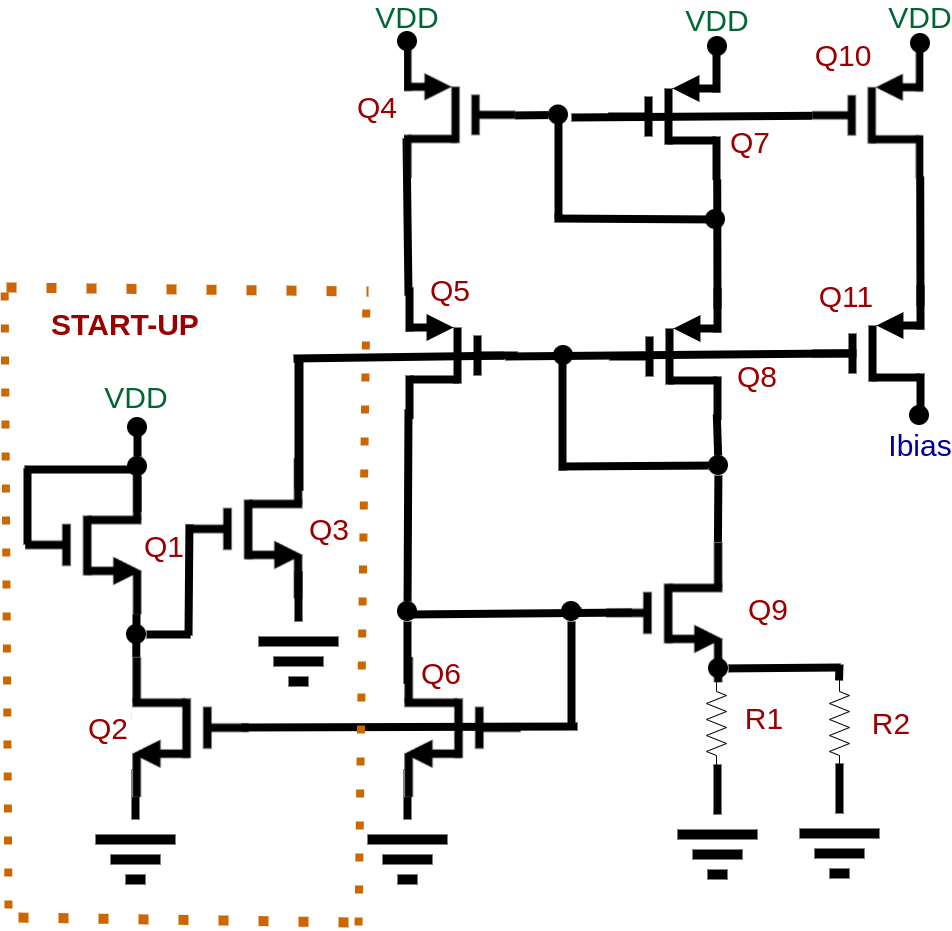
\includegraphics[scale=0.3]{Circuitos/Ibias_generator.png}
    \legend{Fonte: Produzido pelo autor}
    \label{\NomePFig}
\end{figure}

\begin{figure}[htb]
 \centering
    \centering
    \caption{\label{\NomeSFig}Representação em bloco do \NomeBloco}
    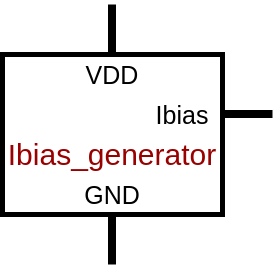
\includegraphics[scale=0.3]{Circuitos/ibias_generator_block.png}
    \legend{Fonte: Produzido pelo autor}
\end{figure}

Os transistores utilizados no bloco apresentam os par\^ametros mostrados na \autoref{\NomeTTab}.

\begin{table}[!h]
\caption{Transistores do Bloco \NomeBloco}
\label{\NomeTTab}
\centering
\begin{tabular}{ccccc}
\toprule
Transistor & W ($\mu$m)  & L ($\mu$m)           & M (n° dispositivos) & S (n° dispositivos)\\
\midrule \midrule
Q1 & 0,3 & 19,995 & 1 & 3\\
\midrule
Q2 & 25 & 0,5 & 2 & 1\\
\midrule
Q3 & 30 & 0,5 & 1 & 1\\
\midrule
Q4, Q7 e Q10 & 35 & 4 & 2 & 1\\
\midrule
Q5, Q8 e Q11 & 25 & 2,5 & 2 & 1\\
\midrule
Q6 & 20 & 4 & 2 & 1\\
\midrule
Q9 & 20 & 4 & 4 & 1\\
\midrule
Q10 & 25 & 2,5 & 2 & 1\\
\midrule
Q11 & 25 & 2,5 & 2 & 1\\
\bottomrule
\end{tabular}
\legend{Fonte: Produzido pelo autor}
\end{table}

O resistor utilizado no bloco apresenta os par\^ametros mostrados na \autoref{\NomeQTab}.

\begin{table}[!h]
\caption{Resistor do bloco \NomeBloco}
\label{\NomeQTab}
\centering
\begin{tabular}{ccccc}
\toprule
Resistor & W ($\mu$m)  & L ($\mu$m) & M (n° dispositivos) & Resist\^encia (k$\Omega$)\\
\midrule \midrule
R & 8 & 29,98 & 2 & 0,569025\\
\bottomrule
\end{tabular}
\legend{Fonte: Produzido pelo autor}
\end{table}

Os transistores \textit{Q6} e \textit{Q9}, juntos aos resistores \textit{R1} e \textit{R2}, t\^em a finalidade de funcionarem como um dreno de corrente referenciados pelos resistores. Os transistores \textit{Q4} e \textit{Q7} t\^em a finalidade de funcionarem como uma fonte de corrente, referenciados pelo dreno de corrente j\'a mencionado. O transistor \textit{Q10} \'e o braço do espelho de corrente do qual fornece a corrente de sa\'ida.

Os transistores \textit{Q5}, \textit{Q8} e \textit{Q11} se apresentam na configuração \textit{Cascode}, que tem o intuito de tornar o espelho de corrente de resposta mais linear, aumentar sua banda e ainda aumentar as suas resist\^encias de entrada e sa\'ida.

Os transistores \textit{Q1}, \textit{Q2} e \textit{Q3} t\^em a função de inicializar o circuito no ponto de operação adequado, j\'a que o circuito tamb\'em apresenta estabilidade quando fornecendo 0 A, sendo necess\'ario evitar essa situação.
